\documentclass[10pt,a4paper]{article}
\usepackage[margin=15mm,bottom=20mm]{geometry}
\usepackage{fontspec,xeCJK}
\setmainfont{Arial}
\setCJKmainfont{Microsoft YaHei}
\usepackage{graphicx,tikz,longtable,array,booktabs,amssymb,setspace,titlesec,fancyhdr,lastpage,hyperref}
\hypersetup{hidelinks,pdftitle={HollowHaven Technical Manual}}
\setstretch{1.65}
\setlength{\parindent}{0pt}\setlength{\parskip}{7pt}
\setlength{\emergencystretch}{3em}
\titleformat{\section}{\Large\bfseries}{\thesection.}{.5em}{}[\vspace{5pt}\titlerule]
\titleformat{\subsection}{\large\bfseries}{\thesubsection}{.5em}{}
\titlespacing*{\section}{0pt}{20pt}{12pt}
\titlespacing*{\subsection}{0pt}{16pt}{8pt}
\renewcommand{\arraystretch}{1.3}
\pagestyle{fancy}\fancyhf{}\renewcommand{\headrulewidth}{0pt}
\fancyfoot[C]{\fontsize{6}{8}\selectfont HollowHaven · \thepage\ / \pageref*{LastPage}}
\begin{document}
\thispagestyle{empty}
\begingroup
\definecolor{coverink}{HTML}{283540}
\definecolor{covergray}{HTML}{7C8791}
\setstretch{1}
\vspace*{12mm}
\noindent\hspace*{9mm}{\color{covergray}\fontsize{10}{14}\selectfont H O L L O W H A V E N}\par
\vspace*{64mm}
\noindent\hspace*{9mm}{\color{coverink}\fontsize{34}{42}\selectfont 技术手册}\par
\vspace{8mm}
\noindent\hspace*{9mm}{\color{covergray}\fontsize{8}{12}\selectfont TECHNICAL MANUAL}\par
\vfill
\noindent\hspace*{9mm}{\color{covergray}\fontsize{8}{12}\selectfont 2026.11\hspace{8mm}EDITION 01}\par
\vspace*{18mm}
\endgroup
\clearpage
\setcounter{tocdepth}{1}
\renewcommand{\contentsname}{目录}
\begingroup\setstretch{1.05}\small\tableofcontents\endgroup\clearpage
版本：2026-11-06。中文重编版；技术核对基准：Git e40f8b5。正文按系统概述、技术栈、硬件、软件、结构、装配、测试与复刻组织。未提供的尺寸和实测结果保留待补说明。
\section{项目简介与技术目标}

HollowHaven 是面向大袋鼯人工树洞庇护场景开发的课程原型，探索环境监测、自动滴水和来访事件记录在同一装置中的集成。系统以 ESP32 为控制核心，采集环境与设备状态，通过舵机控制重力供水，并将数据传输至电脑网页供观察与记录。


原型外壳结合 Blender 建模与分层装配，由带通气孔的结构层、毛细导水层和树皮外层构成。结构为入口、传感器与水路提供安装位置；导水材料用于扩散水分，树皮形成外观包覆。


\subsection{三条主要功能链}

\begin{longtable}{p{42mm}p{59mm}p{58mm}}
\toprule
\textbf{功能} & \textbf{输入与处理} & \textbf{输出}\\\midrule\endhead
环境监测 & 温湿度、光照、水位、两点材料湿度等数据采集 & 网页状态、趋势、CSV 记录与维护提示\\
自动滴水 & 有效光照与温度满足条件后启动舵机水阀；定时检查温度 & 重力供水及指令状态；湿度探头辅助检查供水响应\\
来访事件记录 & 连续距离读数确认疑似进入 & 约 30 秒录音、WAV 保存及可选人工发起的音频分析\\
\bottomrule\end{longtable}

\subsection{技术目标与验证范围}

原型的技术目标是打通传感器采集、设备本地控制、局域网传输、电脑存储与网页显示，并把电子系统装入分层外壳。技术评估应检查这些环节是否连贯、可重复且容易维护。


当前材料可以支持说明代码中的功能与照片中的装配关系。本文不据此宣称已验证降温幅度、长期防水性能或野生动物适用性。距离事件与音频分析仅提供观察线索，不能直接确认动物种类。


\subsection{阅读后的预期成果}

读者应能够解释各技术层的作用，按接线表搭建桌面原型，部署指定版本的软件，检查基本功能，并识别完成机械复刻前必须补齐的尺寸与工艺资料。


\clearpage
\section{系统架构与技术栈}

\subsection{系统分工}

\begin{center}
\begin{tikzpicture}[every node/.style={draw,rounded corners,align=center,minimum width=36mm,minimum height=17mm,font=\small}]
\node (a) at (0,0) {传感器与水阀\\采集 / PWM};
\node (b) at (4.2,0) {ESP32 固件\\控制 / 录音};
\node (c) at (8.4,0) {Node.js 服务\\校验 / 存储};
\node (d) at (12.6,0) {浏览器页面\\显示 / 操作};
\draw[->] (a)--(b);\draw[->] (b)--(c);\draw[->] (c)--(d);
\node (e) at (8.4,-2) {可选外部音频分析\\由用户主动发起};
\draw[->] (c)--(e);
\end{tikzpicture}
\end{center}

图 1 系统架构。实线框按数据处理顺序排列；水阀控制在设备端执行，可选音频分析由用户发起。


\begin{longtable}{p{42mm}p{59mm}p{58mm}}
\toprule
\textbf{技术层} & \textbf{当前技术} & \textbf{负责内容}\\\midrule\endhead
硬件 & ESP32-WROOM-32、传感器、MG90S 舵机 & 物理量采集、水阀驱动\\
固件 & C、ESP-IDF、PlatformIO & I²C / ADC 采集、PWM、状态机与录音缓存\\
通信 & Wi-Fi 局域网、UDP、TCP & 设备发现、遥测与音频传输\\
本地服务 & Node.js & 连接设备、协议校验、文件存储与网页接口\\
浏览器 & HTML、CSS、JavaScript & 实时状态、趋势、录音与设置交互\\
数据 & CSV、WAV、JSON & 遥测、音频、分析结果与非敏感设置\\
结构设计 & Blender、分层外壳装配 & 曲面外壳、通气孔、导水与外观包覆\\
\bottomrule\end{longtable}

\subsection{架构选择及运行边界}

设备端独立执行控制逻辑，使阀门决策不依赖网页是否打开。电脑负责接收、保存和展示；断开电脑会中断数据接收，但不会停止设备端控制。当前系统不能补回完整的离线遥测历史。


遥测与音频使用不同 TCP 连接，分别处理状态数据和音频文件。浏览器访问本地 Node.js 服务，并不直接读取传感器。可选音频分析由服务端代理调用，其返回结果不参与水阀决策。


\clearpage
\section{硬件设计与实现}

\subsection{元件组成与用途}

\begin{longtable}{p{42mm}p{59mm}p{58mm}}
\toprule
\textbf{元件} & \textbf{数量} & \textbf{接口与作用}\\\midrule\endhead
ESP32-WROOM-32 开发板及匹配扩展底板 & 各 1 & 采集、控制与 Wi-Fi 通信\\
SHT3x 温湿度模块 & 1 & 第一组 I²C；测量腔体空气温湿度\\
VL53L0X 测距模块 & 1 & 第二组 I²C；入口附近距离检测\\
电容湿度模块 & 2 & ADC；观察导水材料不同位置的湿润响应\\
模拟光照模块、水位模块 & 各 1 & ADC；开阀条件与补水提示\\
SEN0487 麦克风 & 1 & 模拟音频输入与声音统计\\
MG90S 舵机及阀门机构 & 各 1 & PWM 驱动机械水阀\\
水箱、水管、毛细吸水垫、固定件 & 按结构准备 & 重力输水、扩散及机械安装\\
\bottomrule\end{longtable}

采购时应确认完整模块的供电与输出电平，不能用裸芯片直接替代模块。光照、水位、电容湿度模块的具体购买型号，阀体和接插件规格仍需补齐。工具至少包括 USB 数据线、万用表、小螺丝刀、绝缘材料与扎带。


\subsection{供电与接口设计}

ESP32 通过板载 USB 接口接标准稳压 5V USB 电源；传感器采用兼容 3.3V 的模块。MG90S 使用独立稳压 5V 供电支路，并与 ESP32 共地；舵机不接 3V3。电源选型还需结合舵机实际负载和动作时压降验证。


全部模拟输入限制在 0–3.3V，读取 AO 模拟输出。模拟采集使用 ADC1，以避免经典 ESP32 在 Wi-Fi 工作时与 ADC2 的资源冲突。两组 I²C 分别连接温湿度和测距模块，排障时应分组验证。


当前未启用 DS18B20，也未启用水位模块的外部电源开关电路。不能仅因配置文件中保留相关定义就接入或启用这些功能。


\clearpage

\subsection{硬件接线图与逐线表}

\begin{center}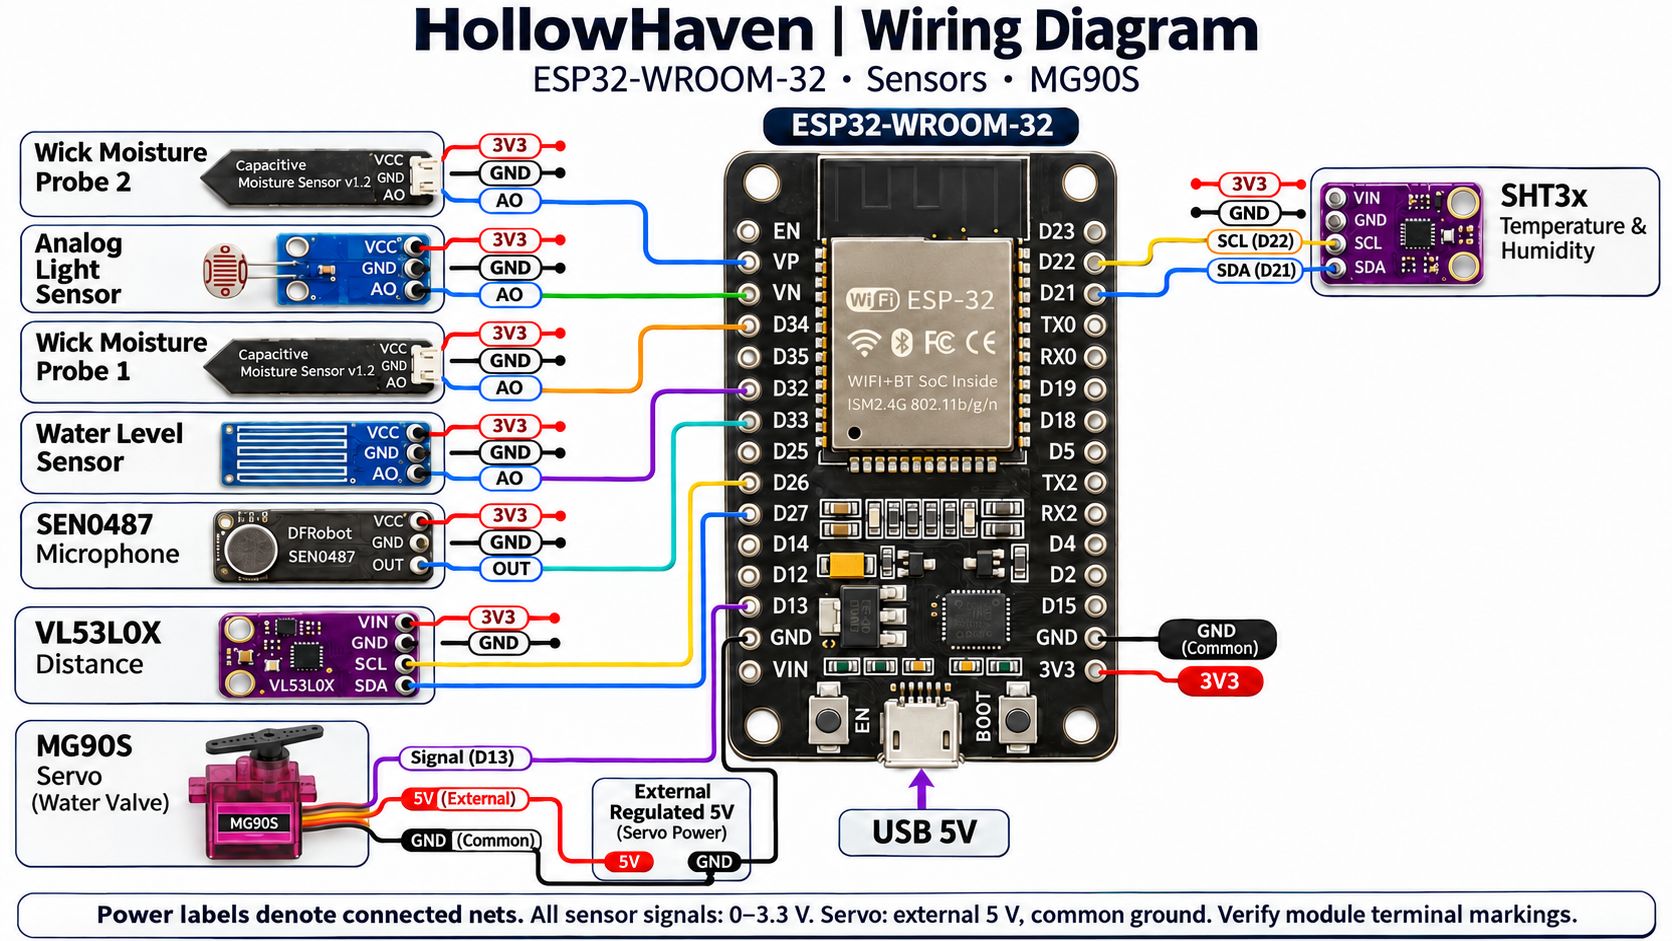
\includegraphics[width=\linewidth,height=90mm,keepaspectratio]{wiring-realistic.png}
\par\small 图 2 原手册接线示意图。线色仅用于识别，接线以模块端子和下表为准。
\end{center}

\begin{longtable}{p{42mm}p{59mm}p{58mm}}
\toprule
\textbf{模块端子} & \textbf{ESP32 / 电源端子} & \textbf{核对要点}\\\midrule\endhead
SHT3x SDA / SCL & GPIO21 / GPIO22 & 第一组 I²C\\
VL53L0X SDA / SCL & GPIO27 / GPIO26 & 第二组 I²C\\
湿度 1 AO & GPIO34 & 第一湿润检测点\\
湿度 2 AO & GPIO36 / VP & 不接 GPIO35 或 VN\\
光照 AO & GPIO39 / VN & 不使用 DO 输出\\
水位 AO & GPIO32 & 原始 ADC，不是毫升值\\
SEN0487 A & GPIO33 & 模拟音频\\
上述传感器 VCC / VIN、GND & 3V3、公共 GND & 确认模块支持 3.3V\\
MG90S 信号、电源正、电源负 & GPIO13、独立 5V、公共 GND & 核对厂家端子标识\\
\bottomrule\end{longtable}

VP 表示 GPIO36，VN 表示 GPIO39，均不是供电极性标记。开发板 D 前缀对应 GPIO 编号；电脑 COM 号则用于烧录连接，与 GPIO 无关。扩展底板的 S/V/G 排列需按实际底板核对，必要时断电测通断；不要依据照片推断被遮挡的线路。


\clearpage

\subsection{传感器与水路工作原理}

SHT3x 提供腔体温湿度，温度参与当前滴水控制。光照、水位和材料湿度以原始 ADC 数值使用；未经标定不能把它们换算为 lux、毫升或含水率。两个湿度点用于观察水是否抵达不同位置，不能证明整个表面都均匀湿润。


VL53L0X 测量入口附近距离，由软件通过连续读数确认疑似进入与离开。SEN0487 提供模拟声音信号，在进入事件后采集音频；麦克风需要与水路和舵机振动源适当隔离。


水路采用“高位水箱—舵机阀门—水管—外部导水层”。水由重力输送，导水材料通过毛细作用扩散，不依赖额外水泵。蒸发效果受温湿度、通风、供水量及材料接触影响，应通过对照测量评估。


\subsection{机械动作与反馈边界}

舵机接收 PWM 指令，经机械耦合带动阀门。当前指令从关闭端到开启端逐步变化，约需 13 秒。网页所示状态来自控制指令；系统没有流量计或阀位反馈，必须用实际出水和材料湿润响应检查动作效果。


初次调试先分离连杆，确认方向和端点，再装回机构。替换舵机、阀体或支架后，重新确定脉宽端点和机械限位，避免卡死。水箱高度、管径和阀体影响实际流量，这些参数需要随装配记录一起保存。


\subsection{本章复刻检查点}

逐根核对信号、供电和地；模拟输出不得超过输入范围；舵机动作时检查 ESP32 是否重启。先完成无水验证，再加水观察实际通路。温湿度探头测腔体空气，湿度探头测导水材料，两者安装位置不能混淆。


\clearpage
\section{软件设计与实现}

\subsection{软件模块与责任}

\begin{longtable}{p{54mm}p{111mm}}
\toprule
\textbf{模块 / 文件位置} & \textbf{主要责任}\\\midrule\endhead
project/firmware/main/ & 设备启动、传感器采集、网络与任务组织\\
sensors.c、analog.c & 数字传感器、模拟量、声音采集\\
presence\_sensor.c、shared/presence.h & 测距事件确认及进出状态\\
servo.c、shared/valve\_control.h & PWM 动作及滴水控制状态\\
audio\_record.c & 音频缓存、录音与传输管理\\
website/protocol.js & 遥测解析与音频校验\\
website/server.js & 连接、存储、网页接口与分析代理\\
website/public/ & 页面、样式、交互与控制状态展示\\
\bottomrule\end{longtable}

设备周期采集传感器数据，维护有效性标志和控制状态，并向电脑输出遥测。软件应区分数值、有效性与数据新鲜度；无效或陈旧数据不能视作正常测量。未接模块的 ADC 浮动值不一定能被软件自动识别。


\subsection{滴水控制逻辑}

关闭状态下，仅当光照数据有效且 ADC＜500，同时温度有效且大于 30°C，才请求开阀。舵机达到指令全开状态后开始计时，至少维持 60 秒。随后每分钟检查一次温度：有效且低于 26°C 时关闭，否则继续保持并等待下一次检查。


开启后的光照变化不终止本轮周期；无效温度不会触发关闭。低水位用于告警，当前没有自动阻止开阀的联锁。以上均为现有实现行为，测试时需要单独覆盖。


开启条件 $\rightarrow$ 舵机渐进动作 $\rightarrow$ 指令全开 $\rightarrow$ 保持 60 秒 $\rightarrow$ 检查温度 $\rightarrow$ 关闭或继续等待。


\clearpage

\subsection{当前参数及校准位置}

\begin{longtable}{p{42mm}p{59mm}p{58mm}}
\toprule
\textbf{项目} & \textbf{当前值 / 行为} & \textbf{复刻注意事项}\\\midrule\endhead
开阀条件 & 有效光照 ADC＜500 且温度＞30°C & 实测遮光 / 照光，确认 ADC 方向\\
关阀条件 & 全开至少 60 秒后，每分钟检查；温度＜26°C & 等于边界值不会满足严格比较\\
舵机 PWM & 50Hz；开 1200μs、关 2500μs & 按阀体校准，不能直接当作角度\\
舵机渐变 & 每 100ms 改变 10μs & 全行程约 13 秒\\
材料湿度 & ADC＜2000 湿；$\geq$2300 干 & 中间区保留前态；初始或无效为未知\\
供水异常提示 & 全开$\geq$60秒且任一点仍干燥 & 仅提示可能异常，需人工检查水路\\
低水位提示 & ADC＜50 & “小于50ml”标签不代表体积标定\\
进入 / 离开 & 连续3次$\leq$189mm / 连续5次$\geq$220mm & 约100ms采样；装入外壳后重测背景距离\\
事件录音 & 约30秒 & 持续停留不不断重触发\\
\bottomrule\end{longtable}

引脚、功能开关及部分阈值位于 project\_config.h；滴水状态逻辑位于 shared/valve\_control.h；材料湿度、维护提示和进出状态分别查看 shared 下的对应模块。阈值变更需修改固件、重新构建烧录，并同步更新校准记录。


\subsection{距离触发与音频缓存}

连续读数确认与不同进出阈值共同减少边界抖动。一次进入事件请求录音，之后将 PCM 数据及元数据发送到电脑。设备 Flash 缓冲有限，离线期间的录音可能被覆盖；不能把本地缓冲视为无限期档案。


音频传输带 CRC32 校验，电脑校验、写出 WAV 后确认接收。CRC32 用于检查传输完整性，不能证明采样没有缺口，也不能证明录音对象的身份。


\clearpage

\subsection{通信与存储}

\begin{longtable}{p{42mm}p{59mm}p{58mm}}
\toprule
\textbf{链路} & \textbf{地址 / 端口} & \textbf{用途}\\\midrule\endhead
设备发现 & UDP 9002 & 电脑在局域网发现 ESP32\\
遥测 & TCP 9000 & 版本头与 CSV 行，含序号、时间及状态\\
音频 & TCP 9001 & 录音元数据、PCM 与校验\\
浏览器访问 & http://127.0.0.1:8766 & 本机 Node.js 服务\\
\bottomrule\end{longtable}

电脑与 ESP32 连接同一路由器。遥测记录包含设备启动标识、序号、运行时间和有效性；电脑另记接收时间，以帮助区分设备时间与接收时刻。发现失败时可根据串口输出手动填写设备 IP。


\begin{longtable}{p{54mm}p{111mm}}
\toprule
\textbf{存储位置} & \textbf{保存内容}\\\midrule\endhead
website/data/session\_*.csv & 服务会话遥测\\
website/recordings/ & WAV 录音\\
website/data/results.json & 音频分析结果\\
website/data/settings.json & 非敏感设置\\
\bottomrule\end{longtable}

\subsection{网页与可选音频分析}

网页提供实时状态、趋势、维护提示、CSV 导出、录音检索、播放、下载及 WAV 导入。趋势显示使用后端最近最多 900 条样本；录音列表展示最近最多 250 个 WAV，这一显示上限不是自动删除规则。


用户选择音频并主动发起分析后，Node.js 调用配置的外部服务。结果仅作待核实候选；API 密钥保存在服务进程内存中，重启后需重新输入。


网页没有手动水阀开关，关闭网页或暂停接收不会修改固件阈值。排障时按“设备采集—网络传输—服务接收—网页显示”分层检查。


\clearpage
\section{3D 建模与机械结构设计}

\subsection{模型结构与设计意图}

结构设计使用 Blender。现有模型截图展示弧形壳体、三角形开孔与连续边缘；开孔为通气提供通道，连续边缘为装配提供结构基础。最终强度和固定方案需要结合实际壁厚、材料及连接方式验证。


\begin{center}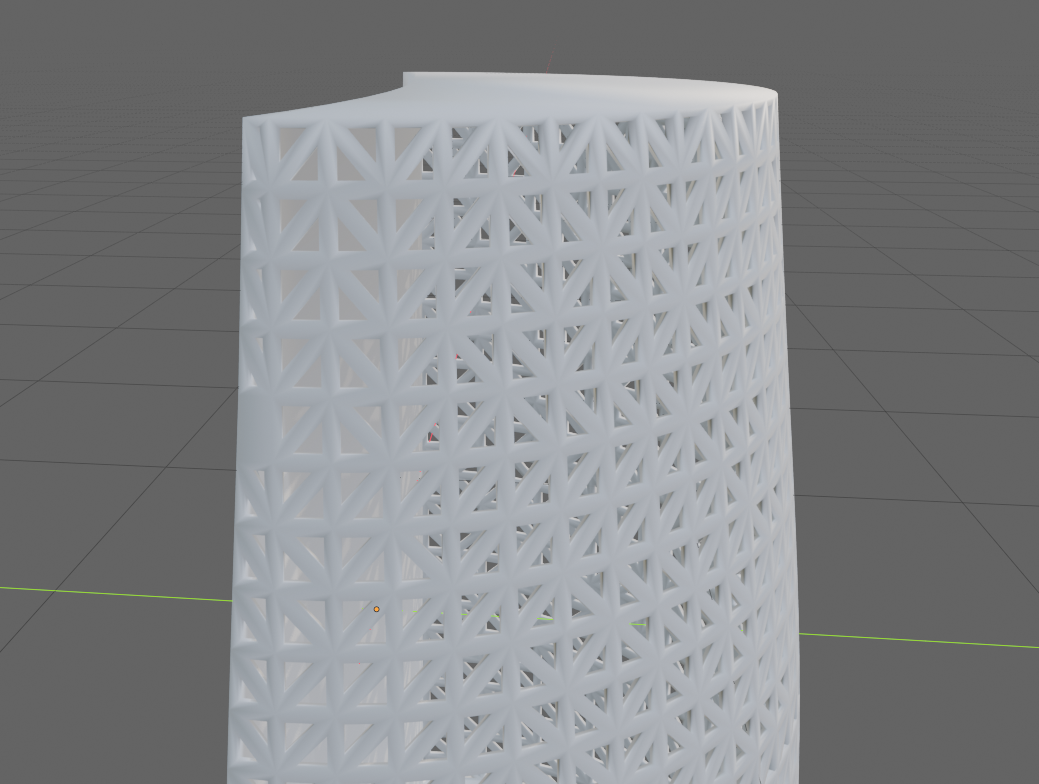
\includegraphics[width=\linewidth,height=68mm,keepaspectratio]{images/M1.png}
\par\small 图 3 透气结构局部：曲面网格与三角形开孔。
\end{center}

\begin{center}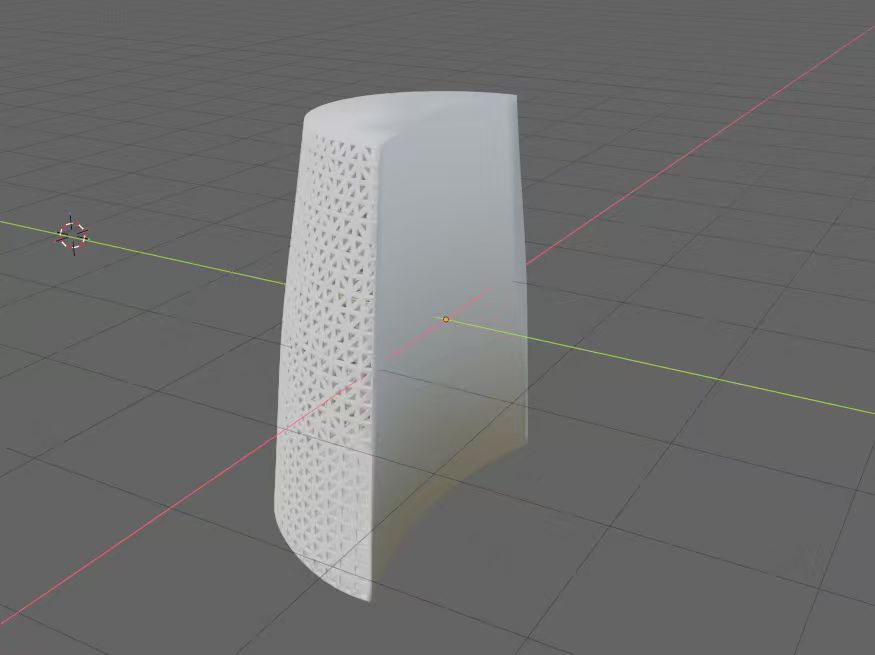
\includegraphics[width=\linewidth,height=68mm,keepaspectratio]{images/M2.jpg}
\par\small 图 4 模型整体视图：弧形壳体、开孔区与边缘。两图均未标注制造尺寸。
\end{center}

仓库 modeling 目录保留 Blender 模型资产。复刻时需核对所用文件与最终实物版本的对应关系，再检查单位、比例和导出网格。图片中的比例不能替代尺寸图。


\clearpage

\subsection{三层结构与安装布局}

由内向外依次为透气结构层、毛细导水层和树皮层。导水层通过连续接触扩散水分；湿层和排水应远离内部休息空间与电子系统。外层固定时应保留入口和必要通气通道。


温湿度探头置于能够反映腔体空气的位置；测距探头视场避开线束和壳体；麦克风避水并远离舵机振动。两处湿度探头放在不同导水位置。水箱、阀体、维修口与线束固定位置需在最终结构图中标明。


\subsection{制造前必须补齐的参数}

\begin{longtable}{p{54mm}p{111mm}}
\toprule
\textbf{对象} & \textbf{待测量或确认的内容}\\\midrule\endhead
主体与顶盖 & 高宽深、壁厚、材料、拆分和连接方式\\
入口与内部空间 & 入口直径、离底高度、有效腔体尺寸\\
通气孔 & 孔径或边长、数量、间距与覆盖区域\\
水箱与水路 & 容量、相对高度、管径、阀体及排水路径\\
舵机与电子仓 & 支架尺寸、孔位、机械限位、维修方式\\
分层材料 & 吸水垫厚度和铺设尺寸、树皮固定方式\\
加工与打印 & 设备、材料、层高、填充、支撑和方向\\
\bottomrule\end{longtable}

本次资料未提供上述完整数值，不能据此输出准确制造图。原手册中的未来全尺寸对标不等于本原型实测尺寸；复刻应以确认后的模型和测量表为准。


\subsection{建模与导出建议}

先确定实际元件和水路的安装空间，再调整外形。检查模型单位、闭合性、壁厚、孔位与装配间隙；打印小型连接试件验证配合后再加工完整主体。保存可编辑的 .blend 文件，并交付适合制造的网格文件及标注尺寸图。具体打印参数应由材料和设备试验确定，不能从截图推断。


\clearpage
\section{外壳制作与整机装配}

\subsection{实物装配参考}

\begin{center}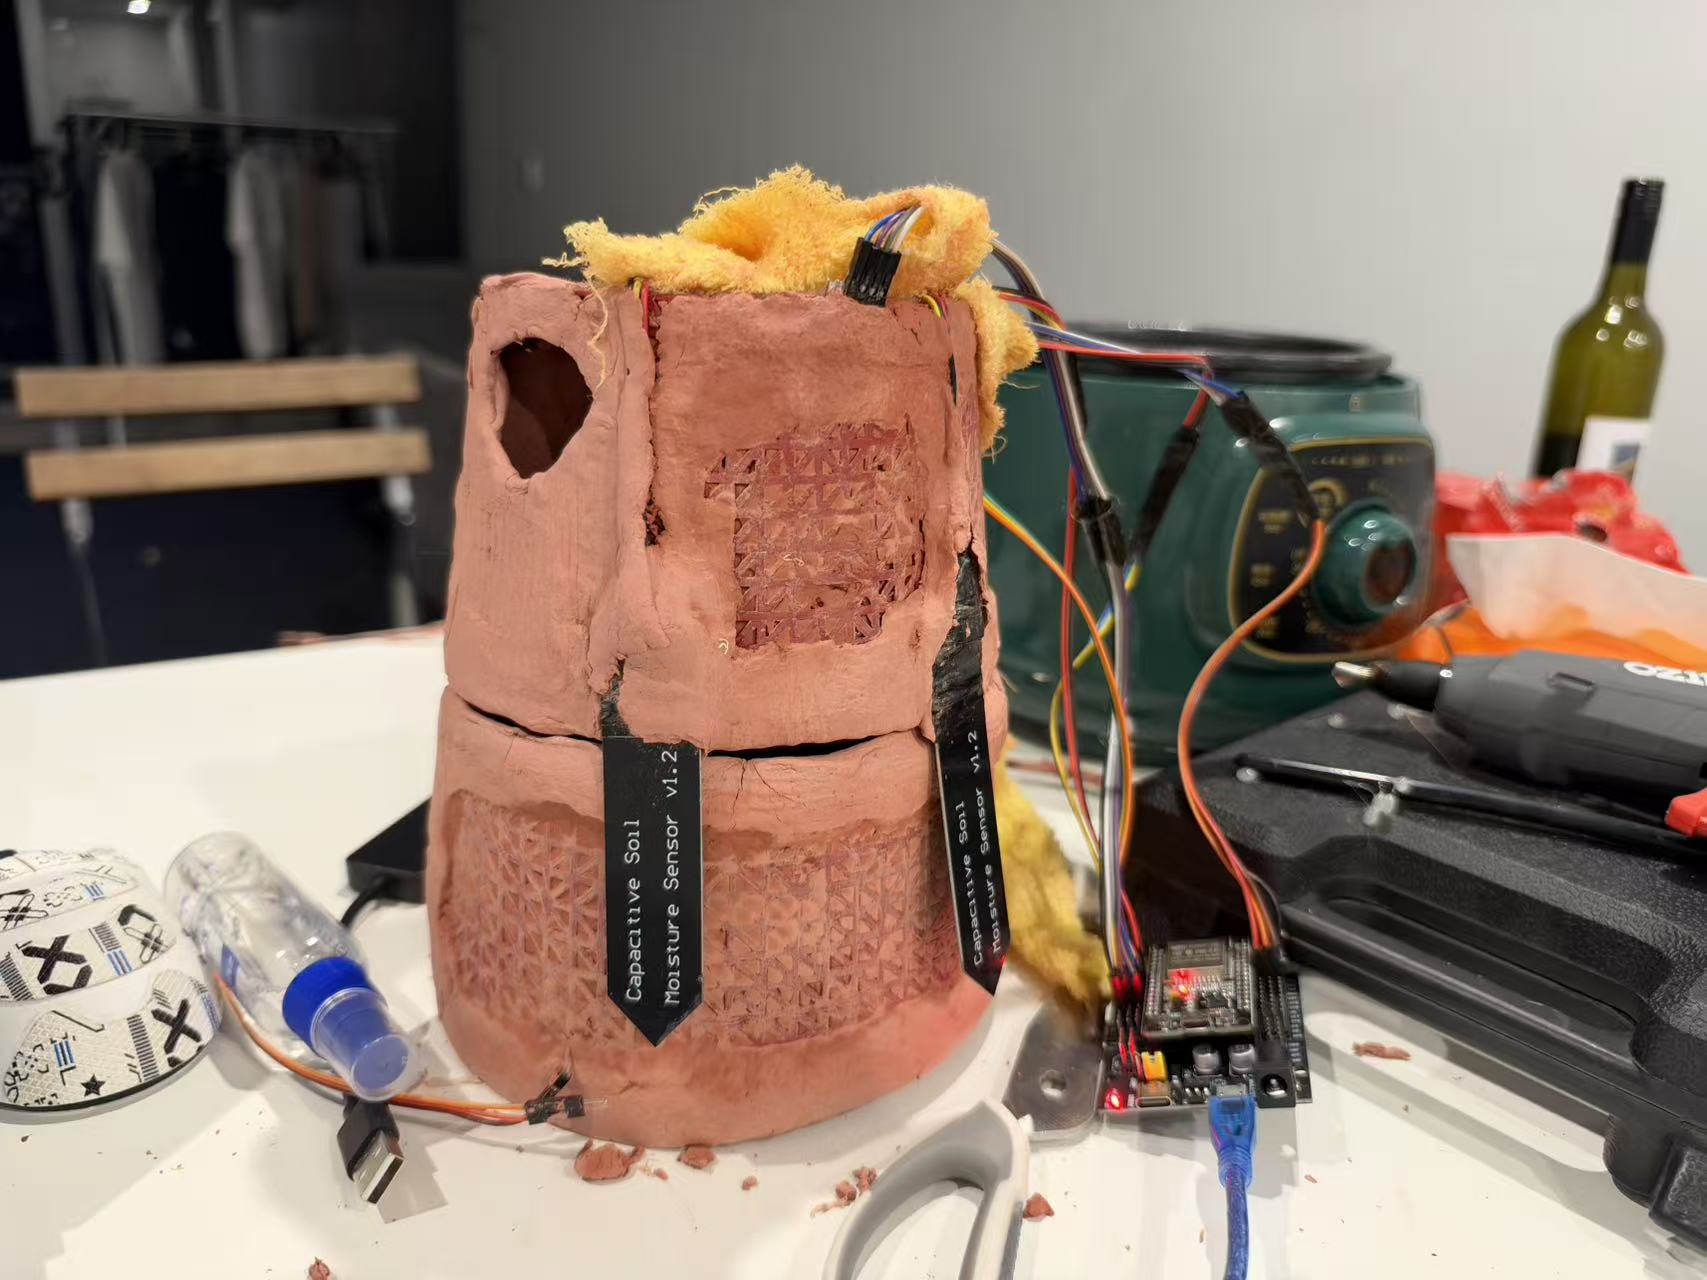
\includegraphics[width=\linewidth,height=68mm,keepaspectratio]{images/M3.jpg}
\par\small 图 5 装配阶段：主体、入口、两处电容湿度探头及外接电子模块。
\end{center}

\begin{center}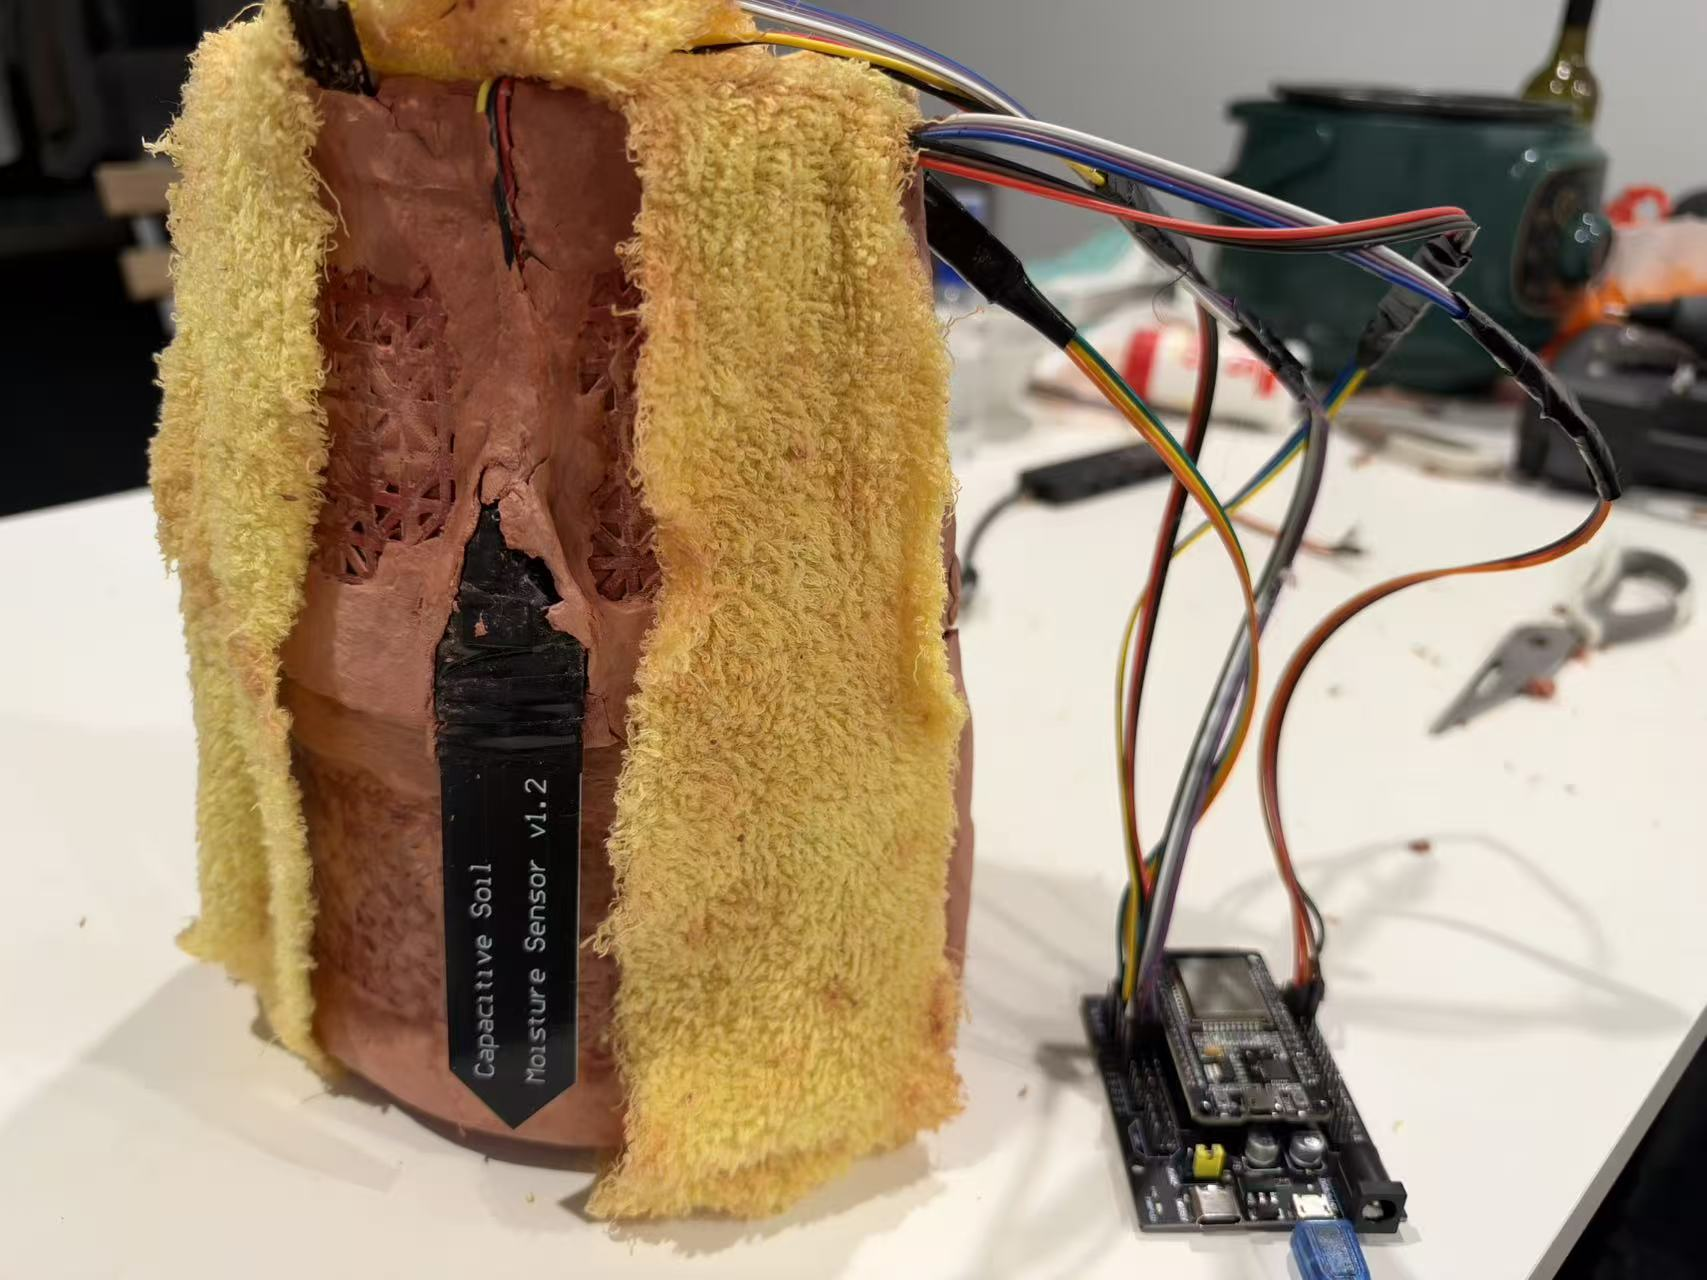
\includegraphics[width=\linewidth,height=68mm,keepaspectratio]{images/M4.jpg}
\par\small 图 6 毛细导水材料铺设阶段：保持材料与结构接触，配合不同位置的湿润检测。
\end{center}

照片用于说明现有原型的装配关系。实际材料成分、粘接剂、紧固方式和防水等级尚未有完整记录，应在复刻前补齐。


\clearpage

\subsection{推荐装配顺序}

\begin{longtable}{p{42mm}p{59mm}p{58mm}}
\toprule
\textbf{阶段} & \textbf{工作内容} & \textbf{完成后检查}\\\midrule\endhead
1 桌面验证 & 接通传感器、固件和网页；舵机先空载 & 数据有效、动作方向正确\\
2 主体处理 & 加工、清理边缘、核对入口和安装空间 & 无毛刺，元件可装入并可维护\\
3 水路干装 & 安装水箱、管路、阀体与舵机支架 & 无干涉，运动不顶住限位\\
4 导水层铺设 & 铺设连续毛细吸水垫并布置两湿度点 & 材料贴合，通气和入口未堵塞\\
5 传感器安装 & 安装温湿度、测距和麦克风 & 测量位置合适，线束不挡视场\\
6 布线固定 & 固定电子模块并整理线束 & 水电分离，连接可靠，保留维修路径\\
7 树皮包覆 & 分块固定树皮并保留入口 & 不压坏线束，不妨碍水路和检修\\
8 注水调试 & 少量加水观察，再进行完整供水周期 & 无渗漏，材料湿润响应可记录\\
\bottomrule\end{longtable}

\subsection{导水层与外壳注意事项}

毛细吸水垫用于扩散水分，效果取决于连续接触、倾斜角度和供水条件。铺设时避免大面积悬空、折叠及堵孔；在预期使用角度检查上部、下部和周向湿润情况。


湿润检测点要保持可重复的接触位置，避免每次拆装改变读数。电子元件的固定、电源接头和水管接头应便于检查；照片中的裸露连线不能作为长期户外安装规范。


完成装配后记录传感器位置、水箱相对高度、管路路线和材料规格，并拍摄包覆前的内部照片，方便维护和下一次复刻。


\clearpage
\section{系统测试与结果记录}

\subsection{当前证据与结果边界}

本次重编核对了现有技术手册、团队图片及仓库中的控制配置与状态逻辑，没有重新进行实物实验。代码提供功能实现证据，照片提供装配证据；两者不能替代整机验收和降温效果测量。以下为建议测试方案，不能标记为已通过结果。


\begin{longtable}{p{42mm}p{59mm}p{58mm}}
\toprule
\textbf{测试项} & \textbf{操作与观察} & \textbf{需保存的结果}\\\midrule\endhead
供电与接线 & 断电核对通断；逐个模块接入；观察舵机动作压降 & 电压、异常重启、接线版本\\
传感器 & 改变光照、湿润、水位与距离；核对温湿度有效性 & 原始 ADC、参考条件及安装位置\\
滴水控制 & 覆盖开关阈值、60秒保持、无效温度与低水位状态 & 指令变化、实际动作与时序\\
水路与导水 & 记录开阀后的出水及两点变湿；改变倾角 & 响应时间、湿润分布、渗漏情况\\
事件与音频 & 进入、持续停留、离开、再次进入 & 事件次数、WAV 时长和可播放性\\
网络与保存 & 保存 CSV / WAV，断连并重启服务 & 文件完整性、恢复过程及数据缺口\\
外壳集成 & 检查遮挡、振动、维修和水电隔离 & 问题照片及整改记录\\
\bottomrule\end{longtable}

\subsection{如何验证降温效果}

如需报告降温效果，应设置可比较的供水与不供水条件，记录环境温湿度、照射或光照条件、风况、供水量、传感器位置及测量时间。保留原始数据，比较同类条件下的腔体温度变化，并记录重复次数和传感器误差。


如果只得到某次温度下降，应报告对应条件与时间段，不推断长期性能。两点湿度变湿只说明材料局部响应，不等于已证明整体降温或均匀供水。


\subsection{测试记录格式}

建议每次记录：日期、操作者、固件提交、元件型号、校准值、安装位置、测试输入、预期行为、实际观察、文件名和结论。当前定量结果待团队补充；未测项目保留“待测”，失败项目保留问题及复测记录。


\clearpage
\section{复刻建议与改进方向}

\subsection{软件部署}

准备 Node.js 18 或以上及 PlatformIO。获取仓库后固定到本手册核对版本；后续版本若改变引脚、协议或阈值，应重新核对对应说明。


\begingroup\small\begin{verbatim}
git clone https://github.com/SMGG2302/comp-5047.git
cd comp-5047
git checkout e40f8b5
\end{verbatim}\endgroup

在 project/firmware/main 中将 wifi\_credentials.example.h 复制为 wifi\_credentials.h，填写本地 2.4GHz 路由器信息。真实凭据不放入共享包。保留项目 partitions.csv，避免改变音频缓存布局。


在 project/firmware 目录执行以下命令。COM7 仅为示例，用设备列表中的实际端口替换。


\begingroup\small\begin{verbatim}
pio run
pio device list
pio run -t upload --upload-port COM7
pio device monitor -p COM7 -b 115200
\end{verbatim}\endgroup

在 website 目录运行以下命令，然后在浏览器打开本机页面。


\begingroup\small\begin{verbatim}
node server.js
http://127.0.0.1:8766
\end{verbatim}\endgroup

电脑与 ESP32 接入同一路由器，检查客户端隔离设置，设备地址先选 auto。发现失败时使用串口输出的 IP，并检查 UDP 9002、TCP 9000 / 9001 的连接条件。避免同时运行另一个占用设备接收连接的程序。


首次构建需要下载工具链。Windows 中文路径构建失败时，可参考项目 build-ascii.ps1，但其中本机路径必须按实际电脑调整。


\clearpage

\subsection{分阶段复刻与校准}

建议按“元件准备—桌面接线—固件烧录—服务启动—单模块验证—外壳装配—水路加入—整机测试”推进。每阶段保存结果后再继续，便于定位问题。


先记录材料干燥、湿润及中间状态的 ADC；再验证光照方向、水位阈值和空腔背景距离。舵机端点应在实际机械机构上校准。替换模块或改变位置后，不直接沿用旧阈值。低水位和无效温度行为应纳入复刻测试，不能假设已具备自动保护。


\subsection{常见故障定位}

\begin{longtable}{p{54mm}p{111mm}}
\toprule
\textbf{现象} & \textbf{优先检查}\\\midrule\endhead
找不到 COM 设备 & USB 是否支持数据、驱动、线缆和端口\\
舵机动作时重启 & 供电支路、共地、压降及机械卡死\\
第二路湿度异常 & 是否接到 VP / GPIO36，而非 GPIO35 或 VN\\
I²C 数据无效 & 两组 SDA / SCL、供电与地是否正确\\
模拟数值漂移或极值 & AO 接法、电压范围、接触与模块连接\\
网页找不到设备 & 同一局域网、隔离设置、防火墙、IP 与接收连接\\
开阀后材料仍干燥 & 水箱、堵塞、实际阀位、材料铺设和接触\\
\bottomrule\end{longtable}

\subsection{交付资料与下一步改进}

完整复刻包应包含：版本固定的代码、BOM 与购买型号、接线图、Blender 源文件、制造用模型及尺寸图、打印设置、装配照片、校准表和验收记录。目前优先补齐机械尺寸、固定方式、材料规格及定量测试结果。


后续可评估低水位联锁、温度失效策略、流量或阀位反馈，以及长期供电、排水和户外防护。它们属于改进方向，不属于本文已确认的现有能力。


\subsection{资料依据}

本版基于仓库 SMGG2302/comp-5047 的 e40f8b5 快照，重点核对 project\_config.h、shared/valve\_control.h 和 website/package.json。其余实现说明与图片承接仓库中文版技术手册及技术手册 LaTeX 素材包。仓库地址：https://github.com/SMGG2302/comp-5047。


本版新增的是信息结构、技术解释及复刻组织方式；未将建议测试写成实测结果。制造参数和实验数据补齐后，应更新版本号并保留变更记录。

\end{document}
